%% main.tex — WikiKGQA Challenge @ ISWC 2026 (version française)
%% Compilation : pdfLaTeX
%%
%% Polices : Libertinus Serif (romain), Libertinus Sans (titres), Libertinus
%% Mono (\texttt), Libertinus Math (maths). La classe ceurart charge déjà le
%% paquet `libertinus` qui installe Serif / Sans / Mono. Nous ajoutons ici
%% `libertinust1math` pour accorder les mathématiques.
\documentclass[]{ceurart}

\sloppy

%% --- Polices Libertinus ---------------------------------------------------
%% ceurart.cls charge : \RequirePackage[T1]{fontenc} et \RequirePackage{libertinus}
%% Nous complétons uniquement avec la police mathématique assortie.
\usepackage{libertinust1math}   %% Libertinus Math (type 1, compatible pdfLaTeX)

%% --- Langue ---------------------------------------------------------------
\usepackage[french]{babel}

%% --- Tables et figures ----------------------------------------------------
\usepackage{booktabs}
\usepackage{tabularx}
\usepackage{array}
\usepackage{url}
\usepackage{xcolor}
\usepackage{graphicx}
\graphicspath{{images/}}
\usepackage{siunitx}
\sisetup{group-separator={\,},output-decimal-marker={,}}

\begin{document}

\copyrightyear{2026}
\copyrightclause{Copyright for this paper by its authors.
  Use permitted under Creative Commons License Attribution 4.0 International (CC BY 4.0).}

\conference{WikiKGQA Challenge @ ISWC 2026: International Semantic Web Conference, October 2026, Nara, Japan}

\title{Retrieval TF-IDF d'exemples et sélection guidée par exécution pour la génération few-shot text-to-SPARQL sur Wikidata avec des LLM à pondérations ouvertes}

\tnotemark[1]
\tnotetext[1]{Papier de participation au défi WikiKGQA~@~ISWC~2026, pistes \texttt{en-with-mentions} et \texttt{es-with-mentions}.}

\author[1]{Kenmegne Fokam Emeric Cyrille}[%
orcid=0009-0001-4232-2361,
email=emeric.kenmegne@facsciences-uy1.cm,
]
\cormark[1]

\author[1]{Tela Tela Gilbert Ebenezer}[%
email=gilbert.tela@facsciences-uy1.cm,
]

\address[1]{Department of Computer Science, University of Yaoundé~I, Yaoundé, Cameroun}

\cortext[1]{Auteur correspondant.}

\begin{abstract}
Nous décrivons notre participation aux deux pistes \emph{with-mentions} (anglais et espagnol) du défi WikiKGQA~@~ISWC~2026, dont la tâche consiste à traduire une question en langue naturelle en une requête SPARQL exécutable sur un sous-ensemble de Wikidata. Notre système enchaîne quatre étapes~: un retrieval TF-IDF qui sélectionne trois exemples similaires dans le train, un \emph{prompt few-shot} adressé à un LLM ouvert, une génération de cinq candidats à températures mixtes (un déterministe, quatre à 0{,}7) et une sélection du premier candidat renvoyant un résultat non vide sur l'\emph{endpoint} du défi. Sur le développement (100~questions par langue), nous obtenons F1~macro = 0{,}634 en anglais et 0{,}607 en espagnol~; sur le test officiel Codabench (75~questions par langue), les scores atteignent 0{,}650 et 0{,}630. Une analyse d'erreurs isole deux catégories résistantes~: les questions typées en \emph{«~which~/~qué~»}, qui exigent la chaîne \texttt{P31/P279*} incomplète sur l'\emph{endpoint}, et les requêtes \texttt{COUNT}, pour lesquelles le LLM omet fréquemment l'agrégat. L'ensemble n'utilise que des modèles à pondérations ouvertes (\texttt{gpt-oss-120b}, \texttt{llama-3.3-70b}) accessibles gratuitement via Groq Cloud.
\end{abstract}

\begin{keywords}
  Knowledge Graph Question Answering \sep
  Wikidata \sep
  Large Language Models
\end{keywords}

\maketitle

%==============================================================================
\section{Introduction}
\label{sec:intro}
%==============================================================================
Le \emph{Knowledge Graph Question Answering} (KGQA) vise à interroger un graphe RDF en langue naturelle. Sur un graphe collaboratif comme Wikidata~\cite{vrandecic2014wikidata}, la difficulté est double~: il faut d'abord désambiguïser les mentions vers les bons Q-identifiants, puis traduire la structure logique de la question en un motif de graphe cohérent. Cette seconde étape implique de choisir les bonnes propriétés et de gérer les agrégats, les filtres et les jointures, dans un contexte multilingue. Le défi WikiKGQA~@~ISWC~2026 fournit \num{497}~paires bilingues (anglais~/~espagnol) question–SPARQL adossées au corpus QAWiki, un \emph{endpoint} QLever~\cite{bast2017qlever} servant une vue simplifiée de Wikidata figée pour toute la durée du défi, et une évaluation \emph{online} sur Codabench utilisant la F1 macro QALD~\cite{perevalov2022qald10}. Nous participons aux deux pistes \emph{with-mentions}, dans lesquelles les Q-identifiants des entités mentionnées sont fournis avec la question, ce qui isole la difficulté de la génération de la requête. Nos contributions sont~: (i)~un pipeline en quatre étapes — retrieval TF-IDF, \emph{few-shot prompting}, génération multi-candidate, sélection guidée par exécution — entièrement construit sur des LLM ouverts~; (ii)~une évaluation dev et test des deux pistes, avec F1 macro de 0{,}634~/~0{,}607 sur le dev et 0{,}650~/~0{,}630 sur le test~; (iii)~une analyse d'erreurs structurée qui isole les deux catégories de questions les plus résistantes, à savoir les questions typées et les requêtes \texttt{COUNT}.

%==============================================================================
\section{Travaux connexes}
\label{sec:related}
%==============================================================================
La série QALD~\cite{usbeck2017qald} a fixé le protocole d'évaluation encore utilisé aujourd'hui (F1 macro sur l'union des réponses), et QALD-10~\cite{perevalov2022qald10} a marqué la migration du benchmark vers Wikidata. Les approches classiques par \emph{parsers} sémantiques supervisés ou par \emph{templates} obtiennent de bons résultats sur des distributions vues à l'entraînement mais généralisent mal aux reformulations nouvelles~; la génération \emph{text-to-SPARQL} par un modèle seq2seq entraîné produit une syntaxe correcte mais souffre d'IRI hallucinées — le modèle génère des propriétés plausibles qui n'existent pas dans le graphe cible. Depuis GPT-3~\cite{brown2020gpt3}, plusieurs travaux ont montré qu'un LLM instruit produit des requêtes SPARQL compétitives à partir d'une poignée d'exemples démontrés en contexte~\cite{li2023fewshot}, et KAPING~\cite{baek2023kaping} injecte de plus le voisinage du graphe dans le prompt. Nous héritons de cette lignée le principe du \emph{few-shot prompting} guidé par retrieval, mais choisissons délibérément un retrieveur non appris (TF-IDF~\cite{salton1988term}) pour rester reproductible à partir de ressources publiques. En parallèle, Wang \emph{et al.}~\cite{wang2022selfconsistency} ont popularisé l'idée qu'échantillonner plusieurs sorties et voter améliore la robustesse d'un LLM~; Self-Refine~\cite{madaan2023selfrefine} étend cette famille en demandant au modèle de critiquer puis réécrire sa sortie. Notre sélection guidée par exécution s'inscrit dans cet esprit tout en évacuant l'étape critique~: c'est l'\emph{endpoint} SPARQL lui-même qui joue le rôle d'oracle en séparant les requêtes vides des requêtes exploitables.

%==============================================================================
\section{Tâche et données}
\label{sec:task}
%==============================================================================
Le défi demande, pour chaque question en langue naturelle, la production simultanée d'une requête SPARQL exécutable et de l'ensemble des réponses attendues~: liste de Q-identifiants pour les \texttt{SELECT}, valeur booléenne pour les \texttt{ASK}, entier pour les \texttt{COUNT}. Les organisateurs proposent quatre pistes~: deux avec mentions d'entités fournies (EN et ES), deux sans. Notre soumission couvre les deux pistes \emph{with-mentions}. Le corpus QAWiki est distribué au format JSON dérivé du schéma QALD. Chaque item réunit un identifiant, la question dans les deux langues, la liste des mentions d'entités (label suivi du Q-identifiant), la requête SPARQL de référence et la liste des réponses attendues (Fig.~\ref{fig:dataset}). La version 2026.2 utilisée dans cet article contient \num{497}~questions, réparties selon les splits officiels en \num{317}~train, \num{100}~dev et \num{80}~test (dont 75 effectivement scorées). Le graphe cible est servi par un \emph{endpoint} QLever~\cite{bast2017qlever} spécifique au défi. Ce détail importe~: contrairement à l'\emph{endpoint} public de Wikidata, la vue servie est \emph{simplifiée} et certaines hiérarchies, notamment la fermeture transitive \texttt{P31/P279*}, sont incomplètes~; une requête syntaxiquement parfaite peut donc renvoyer un résultat vide simplement parce que la propriété interrogée n'est pas matérialisée. Nous exploitons ce fait dans la sélection par exécution (Sect.~\ref{sec:method}). La métrique officielle est la F1 macro QALD~\cite{perevalov2022qald10}~: pour chaque question, la F1 est la moyenne harmonique de la précision et du rappel calculés sur l'ensemble des Q-identifiants renvoyés, et le score global est la moyenne des F1 par question. Nous rapportons également, à des fins d'analyse, le nombre de questions parfaitement répondues et complètement ratées.

\begin{figure}[h]
\centering
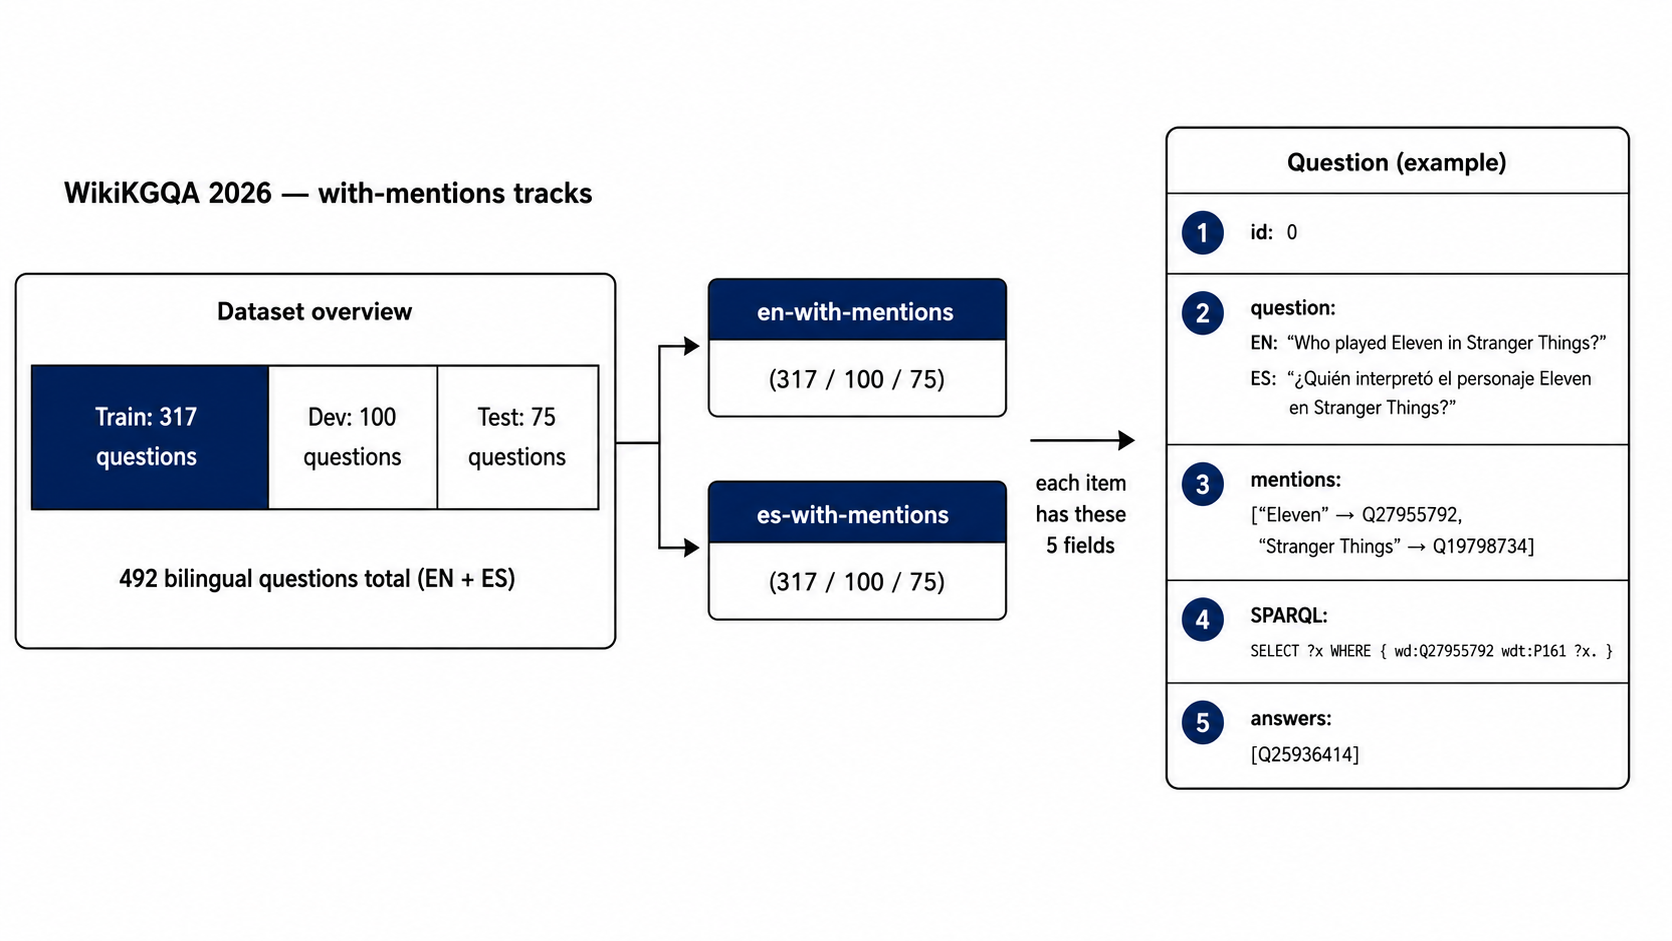
\includegraphics[width=0.9\linewidth]{data.png}
\caption{Format d'un item du corpus QAWiki~: question bilingue, mentions d'entités avec Q-identifiants, requête SPARQL de référence, réponses attendues.}
\label{fig:dataset}
\end{figure}

%==============================================================================
\section{Système proposé}
\label{sec:method}
%==============================================================================
Notre pipeline, désigné P3 dans la suite, est linéaire et n'emploie ni agent ni re-ranker appris. Il prend en entrée une question et ses mentions et produit une requête SPARQL avec l'ensemble de ses réponses (Fig.~\ref{fig:pipeline}). Le retrieval sélectionne, pour chaque question cible, les trois voisins les plus proches dans le train au sens du cosinus entre vecteurs TF-IDF~\cite{salton1988term} construits sur des $n$-grammes de mots avec $n\in\{1,2\}$~; une heuristique légère infère le type de requête cible (\texttt{ASK}, \texttt{COUNT}, \texttt{SELECT}) à partir des interrogatifs et privilégie, à similarité comparable, les voisins de même type. Le vectoriseur s'entraîne en moins d'une seconde sur les \num{317}~questions du train. Le prompt est composé de trois blocs (Fig.~\ref{fig:processing})~: une consigne système qui fixe le format attendu et interdit les déclarations \texttt{PREFIX} (elles seront ajoutées automatiquement à l'exécution)~; les trois exemples formatés en triplets \texttt{(question, mentions, SPARQL)}, chacun clos par un \emph{fenced block} \texttt{```sparql~\dots~```}~; la question cible et ses mentions sous le même format. Pour chaque question, nous interrogeons le LLM cinq fois~: un premier appel à température nulle (pari le plus probable) puis quatre appels à température 0{,}7 (diversification). Chaque candidat est extrait de son bloc de code, préfixé automatiquement par les déclarations \texttt{PREFIX} usuelles de Wikidata, puis soumis à l'\emph{endpoint} via une requête HTTP avec un délai maximum de 30~secondes~; les codes 429 et 5xx sont gérés par une couche de \emph{retry} adaptatif respectant le \texttt{Retry-After} de Groq. La règle de sélection est simple~: nous parcourons les candidats dans l'ordre (déterministe d'abord, puis stochastiques) et renvoyons les réponses du premier candidat qui produit au moins une ligne. Si tous les candidats renvoient un ensemble vide, nous conservons la sortie déterministe, ce qui couvre les rares cas où la réponse de référence est effectivement vide (\texttt{ASK} négatif, \texttt{SELECT} avec \texttt{MINUS}). Le pipeline ne différencie pas les deux langues au niveau du code~: le retrieveur, le format du prompt et la logique de sélection sont identiques~; TF-IDF construit toutefois deux vocabulaires distincts, un par langue.

\begin{figure}[h]
\centering
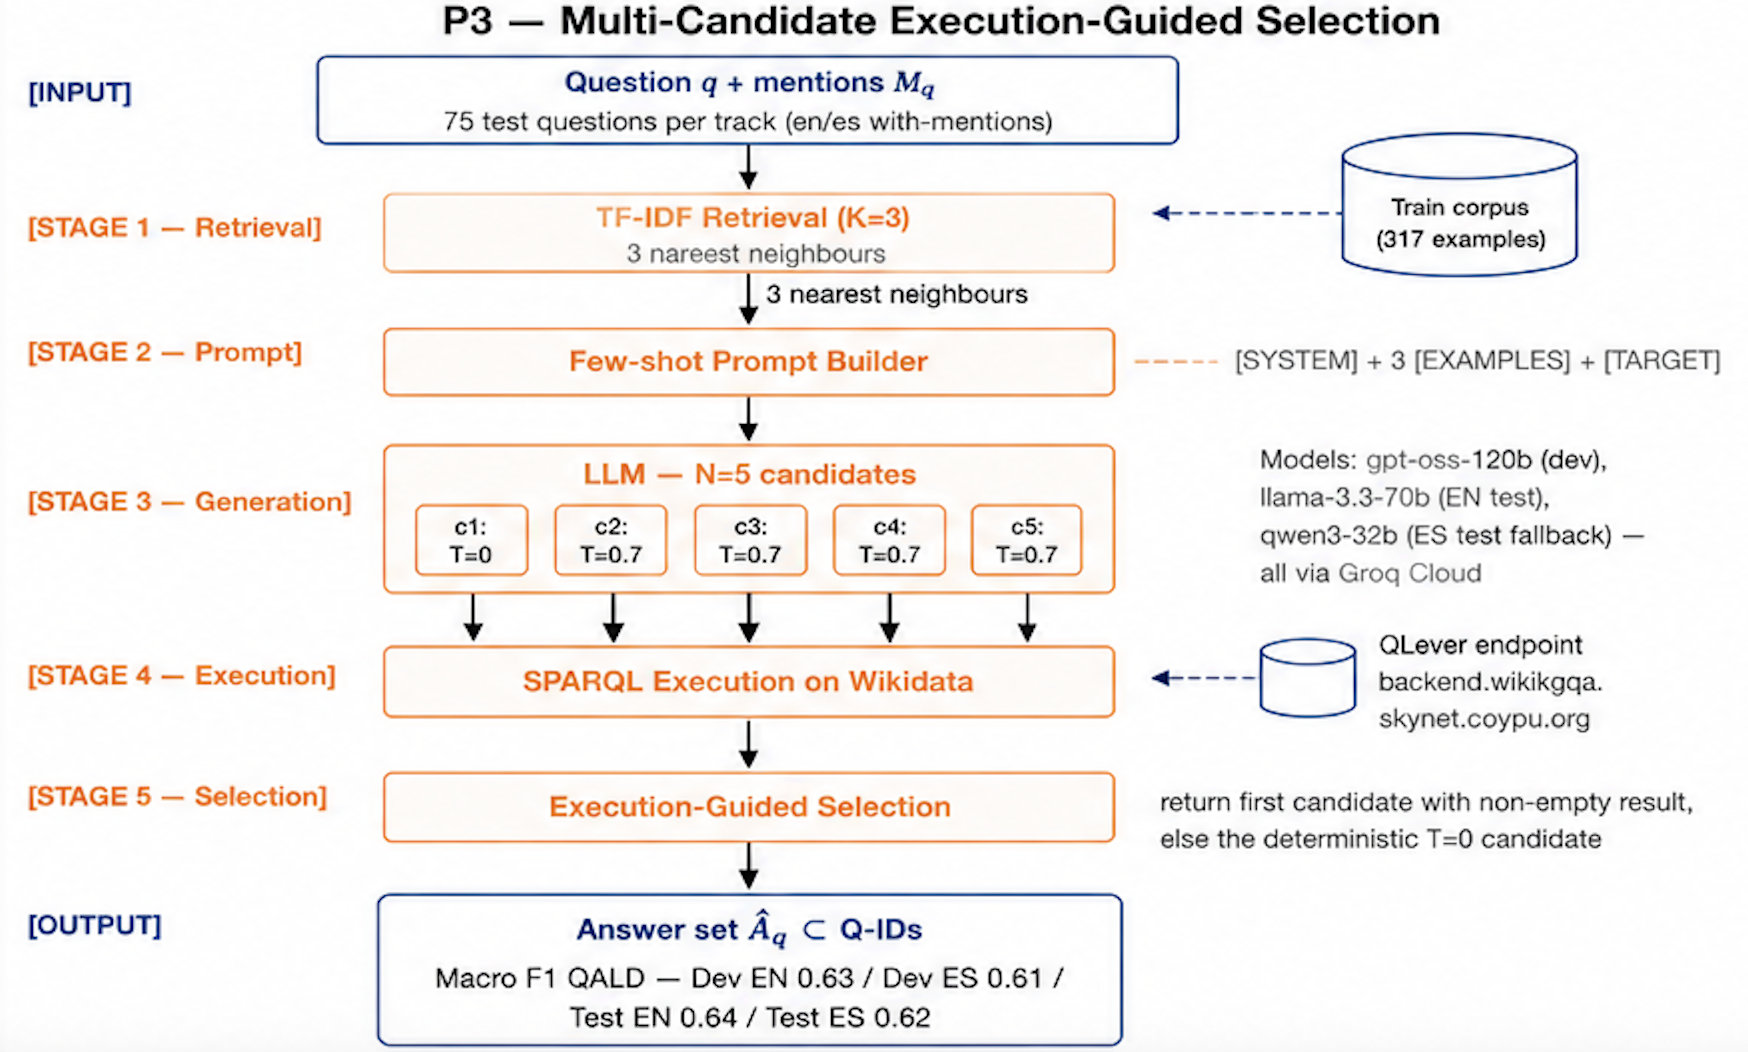
\includegraphics[width=0.78\linewidth]{solution.png}
\caption{Pipeline P3. (1)~Retrieval TF-IDF des trois voisins les plus proches~; (2)~construction du \emph{prompt few-shot}~; (3)~génération de cinq candidats SPARQL par le LLM (un à température 0, quatre à 0{,}7)~; (4)~exécution de chaque candidat sur l'\emph{endpoint} du défi~; (5)~sélection du premier candidat non vide.}
\label{fig:pipeline}
\end{figure}

\begin{figure}[h]
\centering
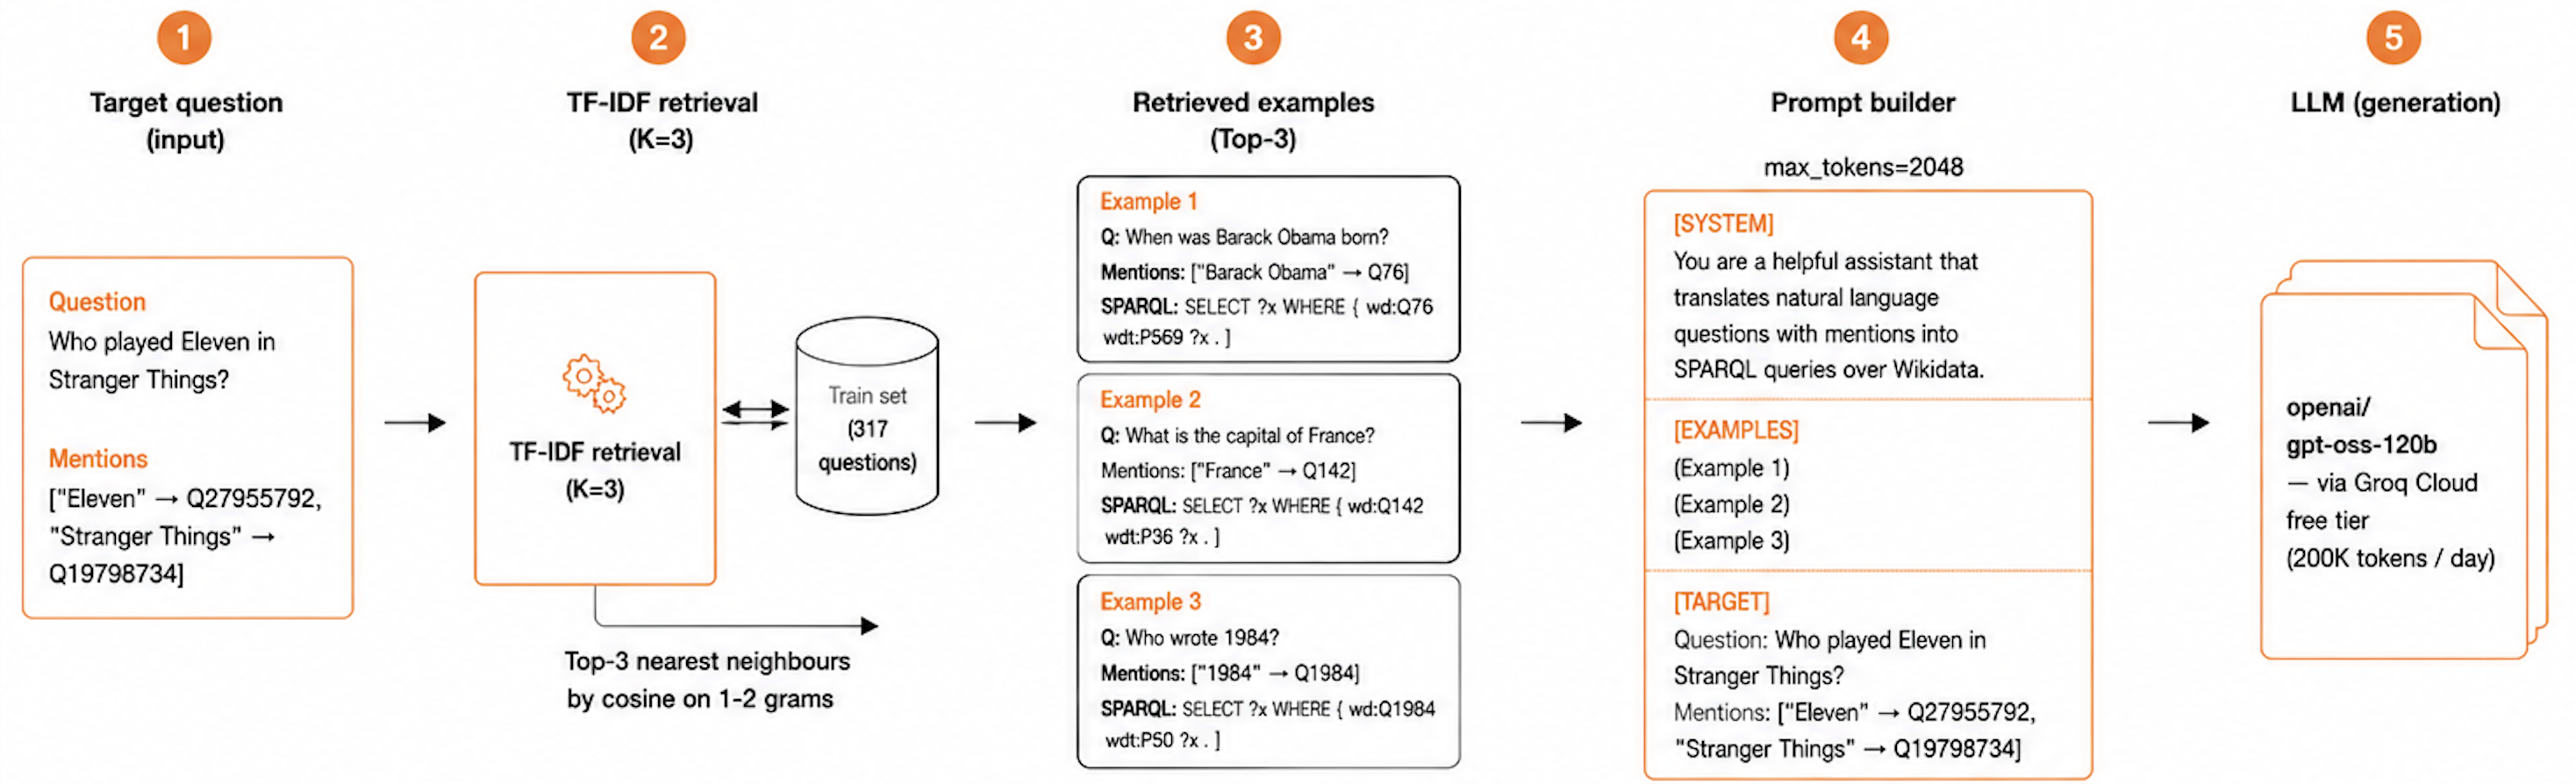
\includegraphics[width=0.95\linewidth]{processing.png}
\caption{Construction du \emph{prompt few-shot}. La question cible et ses mentions déclenchent un retrieval TF-IDF sur les \num{317}~exemples du train~; les trois voisins retenus sont concaténés à la consigne système et à la cible avant envoi au LLM.}
\label{fig:processing}
\end{figure}

%==============================================================================
\section{Protocole expérimental}
\label{sec:setup}
%==============================================================================
Nous utilisons les splits officiels (\num{317}~train, \num{100}~dev, \num{80}~test dont 75 effectivement scorées, pour un total de \num{497}~questions par langue) et évaluons avec la F1 macro QALD définie plus haut. Deux LLM à pondérations ouvertes servent nos expériences~: \texttt{openai/gpt-oss-120b}~\cite{openai2025gptoss} et \texttt{meta-llama/llama-3.3-70b-versatile}, tous deux accessibles via le \emph{free tier} de Groq Cloud~\cite{groq2024} avec un quota quotidien respectivement de 200~k et 100~k tokens. Tous les scores dev (P3 et \emph{single-shot}) rapportés dans cet article sont produits par \texttt{gpt-oss-120b}. Sur le test, la piste espagnole a également tourné avec \texttt{gpt-oss-120b}~; pour la piste anglaise en revanche, le quota quotidien TPD de \texttt{gpt-oss-120b} avait été consommé par les itérations dev de la journée, si bien que nous avons basculé sur \texttt{llama-3.3-70b-versatile} pour rester dans une enveloppe gratuite. Les hyperparamètres sont fixés à $K=3$~voisins retrouvés, $N=5$~candidats générés, séquence de températures $(0{,}0;\,0{,}7;\,0{,}7;\,0{,}7;\,0{,}7)$, un plafond de 2048~tokens par appel et un délai de 6~secondes entre appels pour respecter la limite par minute de Groq. Le baseline de référence est la variante \emph{single-shot} de P3, dans laquelle seul le premier candidat déterministe est produit. Nous n'incluons pas de comparaison à un \emph{parser} sémantique appris car aucun baseline entraîné n'est fourni par les organisateurs. Toutes les expériences se sont déroulées sur un ordinateur portable standard sans GPU, la charge d'inférence étant reportée sur les serveurs de Groq. Grâce à l'arrêt anticipé de la sélection guidée par exécution (75~\% des questions sont résolues dès le premier candidat, cf.~Sect.~\ref{sec:discussion}), le nombre moyen d'appels LLM par question tombe à environ deux et un \emph{dev pass} complet prend 15 à 20~minutes, plutôt que les 50~minutes qu'imposerait un budget systématique de cinq candidats. Un pré-test a vérifié que notre implémentation locale de la métrique reproduit exactement le score renvoyé par Codabench sur les soumissions dev, ce qui autorise à itérer localement avant chaque upload.

%==============================================================================
\section{Résultats}
\label{sec:results}
%==============================================================================
La table~\ref{tab:main} rassemble les scores sur le développement et sur le test officiel Codabench, et la Fig.~\ref{fig:results} en propose une lecture visuelle. Le multi-candidate apporte un gain de +8{,}2~points de F1 en anglais et de +1{,}6~point en espagnol~; l'asymétrie s'explique par la borne inférieure~: en espagnol, le candidat déterministe seul atteint déjà 0{,}591, ce qui laisse moins de marge de rattrapage. Les scores test (0{,}650 en anglais, 0{,}630 en espagnol) sont en parité étroite avec ceux du dev, ce qui indique l'absence de surapprentissage à la distribution de développement.

\begin{table}[h]
\centering
\caption{F1 macro sur le développement (100~questions) et le test officiel (75~questions scorées) des deux pistes \emph{with-mentions}. La variante \emph{single-shot} sert de borne inférieure. Toutes les variantes dev sont produites par \texttt{gpt-oss-120b}~; l'ensemble des scores est arrondi à trois décimales.}
\label{tab:main}
\begin{tabular}{llccc}
\toprule
Piste & Méthode (LLM)                                  & F1 macro & Parfait & Nul \\
\midrule
EN dev  & Single-shot (N=1, gpt-oss-120b)              & 0{,}552 & 52 & 40 \\
EN dev  & P3 multi-candidate (gpt-oss-120b)            & 0{,}634 & 60 & 31 \\
ES dev  & Single-shot (N=1, gpt-oss-120b)              & 0{,}591 & 55 & 37 \\
ES dev  & P3 multi-candidate (gpt-oss-120b)            & 0{,}607 & 56 & 34 \\
\midrule
EN test & P3 multi-candidate (llama-3.3-70b)           & 0{,}650 & — & — \\
ES test & P3 multi-candidate (gpt-oss-120b)            & 0{,}630 & — & — \\
\bottomrule
\end{tabular}
\end{table}

\begin{figure}[h]
\centering
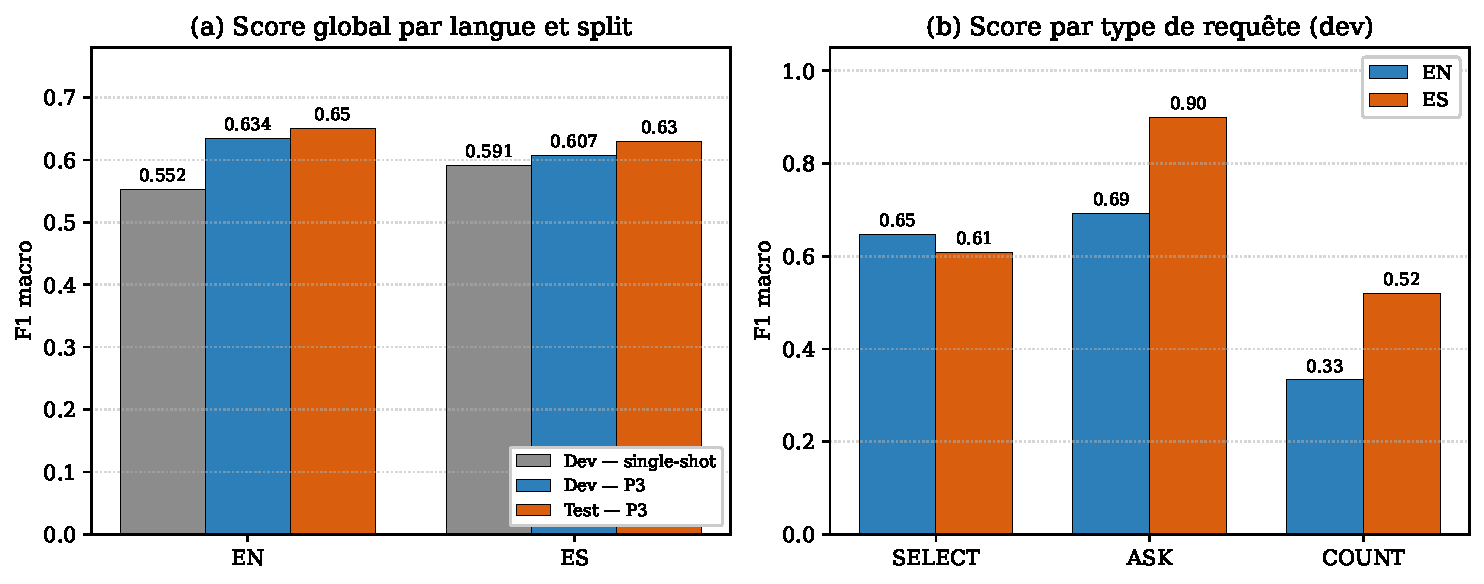
\includegraphics[width=0.95\linewidth]{results.pdf}
\caption{Résultats de P3. (a)~F1 macro par langue et par split~: le multi-candidate est plus rentable en anglais qu'en espagnol, et le test est en parité étroite avec le dev. (b)~F1 par type de requête sur le développement~: les \texttt{ASK} sont bien traités (spécialement en espagnol), les \texttt{COUNT} restent le point faible.}
\label{fig:results}
\end{figure}

Pour quantifier la fragilité du retrieveur aux paraphrases, nous mesurons également le chevauchement Jaccard entre les voisinages top-3 renvoyés par TF-IDF et ceux de trois encodeurs de phrases modernes (\texttt{all-MiniLM-L6-v2}, \texttt{bge-small-en-v1.5}, \texttt{bge-m3}~\cite{chen2024bge}). Le Jaccard moyen oscille autour de 0{,}20 dans les trois cas, ce qui signifie qu'un remplacement par un retrieveur neuronal reconstruirait massivement le contexte few-shot~; c'est notre principale piste d'amélioration.

%==============================================================================
\section{Discussion}
\label{sec:discussion}
%==============================================================================
Nous croisons les prédictions de P3 avec le type de requête généré et le mot interrogatif dominant (Table~\ref{tab:bytypeinterr}). Les deux vues ne se recouvrent pas parfaitement — le bloc supérieur classe les questions selon le type SPARQL effectivement produit par P3, alors que le bloc inférieur les classe selon leur forme de surface (mot interrogatif). Un écart léger entre \emph{how-many/cuántos} et \texttt{COUNT} en est la trace directe~: certaines questions en \emph{«~which~»} demandent en réalité un compte (\emph{«~which country has the most~\ldots ?~»}) et produisent une SPARQL de type \texttt{COUNT}. Les \texttt{COUNT} sous-performent dans les deux langues~; le mode d'échec récurrent est l'oubli de l'agrégat, le LLM produisant \texttt{SELECT ?c WHERE \{~\dots~\}} au lieu de \texttt{SELECT (COUNT(?c) AS ?n) WHERE \{~\dots~\}}. À l'inverse, les \texttt{ASK} en espagnol atteignent 0{,}900~: les formulations oui/non en espagnol (\emph{«~¿Es~\ldots ?~»}, \emph{«~¿Tiene~\ldots ?~»}) sont plus formellement contraintes qu'en anglais, ce qui guide bien le modèle. L'observation la plus nette est structurellement identique dans les deux langues~: une seule catégorie d'interrogatifs concentre la moitié des nuls. En anglais, les \emph{«~which~»} pèsent 32~\% du dev et 15~nuls sur 31~; en espagnol, les \emph{«~qué~»} pèsent 39~\% et 16~nuls sur 34. Ces deux catégories partagent la même structure logique~: filtrer un ensemble d'entités par leur type, ce qui passe par la chaîne \texttt{?x wdt:P31/wdt:P279* wd:Qtype}~; or, cette fermeture transitive est incomplète sur l'\emph{endpoint} du défi. Le LLM génère la chaîne plausible mais l'exécution renvoie zéro ligne. À l'inverse, les questions courtes reposant sur une propriété directe (\emph{«~when~/~cuándo~»}, \emph{«~who~/~quién~»}) sont quasi-parfaites parce qu'elles reposent sur des propriétés bien matérialisées comme \texttt{P569} (date de naissance) ou \texttt{P161} (distribution). Deux gradients complémentaires confirment ce diagnostic~: la F1 chute d'environ 0{,}30~point entre les questions à deux mentions et celles à trois ou plus, et de 0{,}16~point entre les questions courtes ($\leq 6$~mots) et moyennes (7--10~mots), les deux effets convergeant avec la catégorie \emph{«~which~/~qué~»} plus longue et plus contrainte en moyenne. Enfin, la rentabilité du multi-candidate se répartit en trois régimes~: environ 75~\% des questions sont résolues dès le premier tir~; les essais 2 à 4 rattrapent efficacement en anglais (F1 moyenne autour de 0{,}87) mais peu en espagnol (F1 moyenne autour de 0{,}30)~; lorsque les cinq candidats renvoient tous vide, le rattrapage est nul et ces 16 à 18~questions par langue correspondent au profil homogène des chaînes \texttt{P31/P279*}. Trois directions se distinguent pour la suite~: un retrieveur neuronal (\texttt{bge-m3}) pour capter les paraphrases~; un profilage léger de l'\emph{endpoint} — une requête \texttt{SELECT ?p (COUNT(?o) AS ?n)} par entité mentionnée — pour fournir au LLM la liste des propriétés effectivement disponibles~; un tour de raffinement conditionnel à la Self-Refine~\cite{madaan2023selfrefine} sur les seuls cas où les cinq candidats renvoient vide.

\begin{table}[h]
\centering
\caption{Performance par type de requête SPARQL produit par P3 (bloc supérieur) et par mot interrogatif dominant (bloc inférieur) sur les 100~questions du dev EN et ES. Le bloc supérieur totalise 100 questions par langue~; le bloc inférieur omet la catégorie \emph{other} (5 questions en EN, 9 en ES) qui regroupe des interrogatifs marginaux.}
\label{tab:bytypeinterr}
\begin{tabular}{lcccccc}
\toprule
 & \multicolumn{3}{c}{EN} & \multicolumn{3}{c}{ES} \\
\cmidrule(lr){2-4}\cmidrule(lr){5-7}
Catégorie & $n$ & F1 & Nul & $n$ & F1 & Nul \\
\midrule
\multicolumn{7}{l}{\emph{Par type de requête SPARQL}} \\
SELECT   & 81 & 0{,}647 & 23 & 77 & 0{,}584 & 27 \\
ASK      & 13 & 0{,}692 &  4 & 10 & 0{,}900 &  1 \\
COUNT    &  6 & 0{,}333 &  4 & 13 & 0{,}520 &  6 \\
\midrule
\multicolumn{7}{l}{\emph{Par mot interrogatif dominant}} \\
which~/~qué        & 32 & 0{,}425 & 15 & 39 & 0{,}470 & 16 \\
what~/~cuál        & 23 & 0{,}701 &  6 &  9 & 0{,}667 &  3 \\
who~/~quién        & 13 & 0{,}822 &  1 & 13 & 0{,}800 &  2 \\
when~/~cuándo      &  9 & 1{,}000 &  0 &  9 & 0{,}889 &  1 \\
how-many~/~cuántos &  5 & 0{,}200 &  4 & 10 & 0{,}400 &  6 \\
yes-no             & 13 & 0{,}692 &  4 & 10 & 0{,}900 &  1 \\
\bottomrule
\end{tabular}
\end{table}

%==============================================================================
\section{Conclusion}
\label{sec:conclusion}
%==============================================================================
Nous avons présenté un pipeline volontairement simple pour la conversion question-à-SPARQL sur Wikidata, appliqué aux deux pistes \emph{with-mentions} du défi WikiKGQA~@~ISWC~2026. En enchaînant un retrieval TF-IDF, un prompt \emph{few-shot} de trois exemples, une génération de cinq candidats à températures mixtes et une sélection guidée par l'exécution sur l'\emph{endpoint} du défi, le système atteint une F1 macro de 0{,}634 en anglais et 0{,}607 en espagnol sur le développement, et respectivement 0{,}650 et 0{,}630 sur le test officiel Codabench, en n'utilisant que des LLM à pondérations ouvertes accessibles gratuitement. L'analyse d'erreurs identifie deux catégories résistantes — les questions typées en \emph{«~which~/~qué~»}, contrariées par la fermeture transitive \texttt{P31/P279*} incomplète sur l'\emph{endpoint}, et les requêtes \texttt{COUNT} pour lesquelles le LLM oublie l'agrégat — et ouvre trois pistes ciblées~: un retrieveur neuronal pour capter les paraphrases, un profilage léger de l'\emph{endpoint} pour éviter les propriétés non matérialisées, et un tour de raffinement conditionnel pour les questions où le multi-candidate a échoué à rattraper la réponse. Le code, les données et les archives Codabench sont publiés à l'adresse \url{https://github.com/emeric-cyrille/wikikgqa-iswc2026}.

%==============================================================================
\bibliography{main}
%==============================================================================

\end{document}
